\documentclass[
	a4paper, % Paper size, use either a4paper or letterpaper
	10pt, % Default font size, can also use 11pt or 12pt, although this is not recommended
	unnumberedsections, % Comment to enable section numbering
	twoside, % Two side traditional mode where headers and footers change between odd and even pages, comment this option to make them fixed
]{LTJournalArticle}

\addbibresource{sample.bib} % BibLaTeX bibliography file

% A shortened article title to appear in the running head, leave this command empty for no running head

% \footertext{\textit{Journal of Biological Sampling} (2024) 12:533-684} % Text to appear in the footer, leave this command empty for no footer text

\setcounter{page}{1} % The page number of the first page, set this to a higher number if the article is to be part of an issue or larger work

%----------------------------------------------------------------------------------------
%	TITLE SECTION
%----------------------------------------------------------------------------------------

\title{Enhancing Search Precision With Embeddings-Based Semantics} % Article title, use manual lines breaks (\\) to beautify the layout

% Authors are listed in a comma-separated list with superscript numbers indicating affiliations
% \thanks{} is used for any text that should be placed in a footnote on the first page, such as the corresponding author's email, journal acceptance dates, a copyright/license notice, keywords, etc
\author{%
	Adarsh Hiremath \\
	NEUROBIO 240: Biological and Artificial Intelligence \\
	ahiremath@college.harvard.edu
}


%----------------------------------------------------------------------------------------

\begin{document}

\maketitle % Output the title section

%----------------------------------------------------------------------------------------
%	ARTICLE CONTENTS
%----------------------------------------------------------------------------------------

\section{1. Introduction}

Embeddings are numerical representations of words, phrases, or documents that capture their semantic meaning in a vector space. They are commonly used in natural language processing applications, including search, recommendation systems, and sentiment analysis. In search, embeddings can efficiently and accurately retrieve relevant documents or web pages based on the similarity of their semantic content to the user's query.

In December 2022, OpenAI released its newest embedding model, \texttt{text-embedding-ada-002}. Open AI claims that \texttt{text-embedding-ada-002} is far more powerful similar models like BERT. However, little work has been done to quantify the differences between \texttt{text-embedding-ada-002} and other machine learning approaches for search. In this paper, I intend to better quantify these differences by doing the following: 
\begin{itemize}
	\item Implementing search with \texttt{text-embedding-ad}
	\texttt{a-002}, BERT, and fuzzy matching. 
	\item Creating a custom dataset of my.Harvard classes and their corresponding data.
	\item Applying those searches to the my.Harvard dataset.
	\item Quantifying the differences between each search method. 
	\item Building a web application to search Harvard classes and releasing it to the Harvard community. 
\end{itemize}

\section{2. Literature Review}

Literature in the field of text embeddings for information retrieval is largely isolated to individual methods, with little work done to compare the effectiveness of different approaches. My paper aims to address this gap by evaluating the performance of three different search methods: \texttt{text-embedding-ada-002}, fuzzy matching, and BERT. To inform my evaluation, I draw on the following papers:


\begin{itemize}
	\item \textit{Text and Code Embeddings by Contrastive Pre-Training} (Neelakantan et al. 2022): an evaluation of unsupervised text embedding models on large-scale semantic search. These researchers measured an improvement of 23.4, 14.7, and and 10.6 percent over MSMARCO, Natural Questions and TriviaQA benchmarks. 
	\item \textit{Neural Text Embeddings for Information Retrieval} (Mitra and Craswell 2017): an overview of text embeddings pre-\texttt{davinci} for natural language tasks and information retrieval. 
	\item \textit{Semantic Search With Sentence-BERT for Design Information Retrieval} (Walsh and Andrade 2022): an overview of sentence-BERT, a modification to BERT that uses siamese networks for sentence embeddings. 
\end{itemize}

The Neelakantan paper forms the basis for my \texttt{text-embedding-ada002} implementation of semantic search. This paper asserts that it is possible to use a single embedding model to do large-scale semantic search. In my experiments, I use \texttt{text-embedding-ada002}  as the single embedding model for semantic search and evaluate it on the my.Harvard classes dataset. 

The Mitra and Craswell paper provided important context about embeddings in general and was helpful for my general understanding of embeddings.

Finally, the Walsh and Andrade paper was greatly helpful for my initial work on the implementation of the BERT-based search. The insighit of passing in the text through a siamese network to determine similarity was particularly helpful. 

\section{3. Dataset}

Several datasets exist for text classification and  aggregation. Initially, I considered testing my semantic search functionality on the following: 
\begin{itemize}
	\item \textit{MS MARCO}: a text dataset with over $1,000,000$ queries and their corresponding saerch results from the Bing search engine. It is commonly used for passage retrieval. 
	\item \textit{The Reuters Corpus}: a text dataset with over $10,000$ articles from Reuters, labeled with categoreis such as "earnings" and "acquisitions."
	\item \textit{CORD-19}: a dataset with over $200,000$ scholarly articles related to COVID-$19$ and other coronaviruses. It is commonly used for information retrieval.
\end{itemize}

However, none of these datasets had queries pre-labeled with "ground truth" about how relevant search responses were. Instead of manually labeling the relevance of search queries for datasets I was unfamiliar with, I opted to use a custom dataset of my.Harvard classes. This dataset contains over $8000$ my.Harvard classes organized in the following JSON format: 

\begin{python}
	{
		"Id": "G0EnBh8",
		"Subject": "AFRAMER",
		"Number": "11",
		"ClassNumber": "13878",
		"CourseId": "123591",
		"Name": "Introduction to African 
		Studies",
		"Desc": "<p>This course introduces 
		students to the rich diversity and 
		complexity of Africa, including 
		its historical dynamics, 
		economic developments, ...",
		"Profs": "Daniel Agbiboa",
		"F22": true,
		"Days": [
		"Th"
		],
		"M": "N",
		"T": "N",
		"W": "N",
		"R": "Y",
		"F": "N",
		"StartTime": "9:45am",
		"EndTime": "11:45am",
		"HasSection": true,
		"Prereq": "Required of 
		concentrators in African 
		Studies track.",
		"SOC": true,
		"Exam": "12/09/2022 2:00 PM",
		"Location": "Cambridge",
		"URL": "https://locator.
		tlt.harvard.edu/course/
		colgsas-123591/2022/fall/13878",
		"AcadOrg": [
		"AAAS",
		"HIST",
		"EMR"
		]
	}
\end{python}

Given that my.Harvard's native search only works with ultra-precise search queries for course titles and course names, applying semantic search to my.Harvard classes appeared to be a far more useful and relevant use case for the Harvard community.

my.Harvard has no consistency for the JSON representing each class, making the scraping operation extremely difficult. For help with generating the dataset, I reached out to the creator of Deez Classes. 

\section{4. Search Implementations}

Each search technique varies in implementation. \texttt{text-embedding-ada-002}, a transformer-based deep learning architecture is utilized along with cosine similarity to measure query and text similarity. The BERT search is implemented using a custom tokenizer, while fuzzy matching uses string-matching algorithms to return results according to a given threshold.

\subsection{4.1 text-embedding-ada-002}

OpenAI's embedding model, \texttt{text-embedding-ad} 
\texttt{a-002}, utilizes a transformer-based deep learning architecture to learn  embeddings. \texttt{text-embedding-ada-002} outperforms the other top models in three standard benchmarks and is useful for working with natural language and code. Semantically similar text is also numerically similar, and the new embeddings endpoint in the OpenAI API provides easy access to the model used to generate embeddings. Although OpenAI offers three families of embedding models - text embeddings text search / similarity, and code search - I only used the base text embedding model for my project.


\begin{figure}[h]
    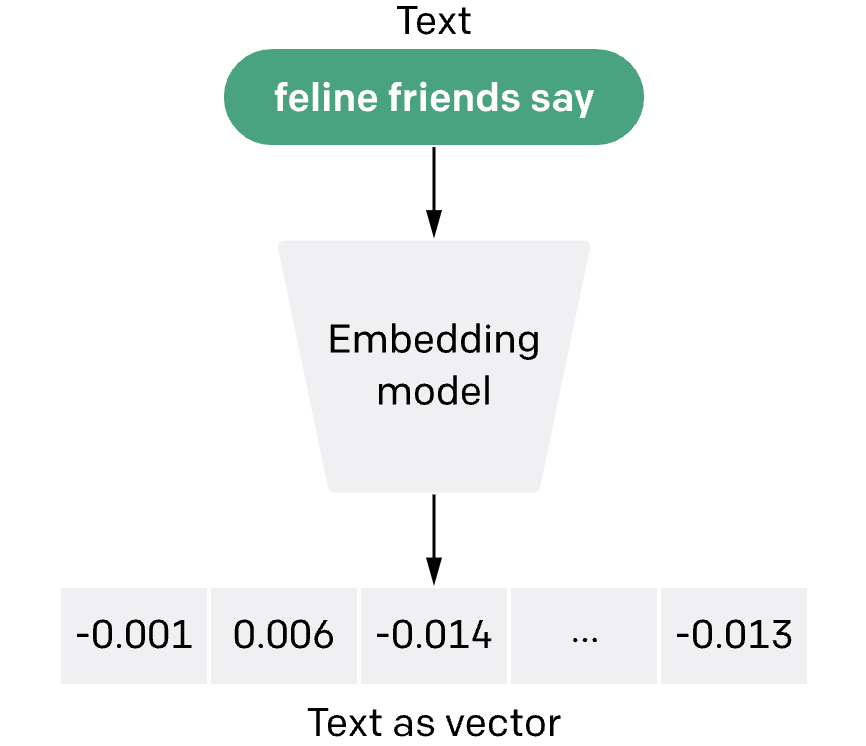
\includegraphics[width=8.1cm]{embedding.png}
    \caption{An example of text embeddings in a vector space.}
    \label{fig:embedding}
\end{figure}


I wanted my search to correctly identify classes based on their name, description, professors, start time, and end time. So, in a Pandas dataframe, I combined all of this information into a column called "combined." From there, generating the embedding was straightforward and required making a call to OpenAI's \texttt{text-embedding-ada-002} endpoint as follows: 

\begin{python}
	course["combined"] = "Title: " + 
	course["Name"] + "; Description: " + 
	course["Desc"] + "; Professors: " + \
	course["Profs"] + "; StartTime: " + \
	course["StartTime"] + "; EndTime: " + 
	course["EndTime"]

	course["embedding"] = 
	openai.Embedding.create(
	input=course["combined"], 
	engine="text-embedding-ada-002")
	["data"][0]["embedding"]
\end{python}

Initially, I considered combining the individual embeddings for the course name, description, professors, start time, and end time to increase the accuracy of my search with a custom formula. However, I decided against this for a couple reasons: 
\begin{itemize}
	\item Dimensionality: it was challenging to combine embeddings because their high dimensionality added an additional alignment step before making meaningful comparisons.
	\item Computational expenses: combining embeddings required calling the Open AI API and doing cosine similarity more times, increasing the cost and time of the algorithm. 
	\item Context: several papers indicated that embeddings can be sensitive to context, leading to variability in their quality and usefulness for different search tasks. Thus, combining embeddings from different sources or models can result in inconsistent or noisy results.
\end{itemize}


\subsection{4.2 BERT}

Just like for the \texttt{text-embedding-ada-002} approach, implementing the BERT search required a similar set of steps: make a combined column, encode the text, and return results by cosine similarity. However, unlike  \texttt{text-embedding-ada-002}, BERT required some additional modifications to work properly. 

BERT expects input in a specific format, where each token is mapped to a unique integer ID, and special tokens are added to denote the start and end of the input sequence. Therefore, before encoding the text using BERT, I need to tokenize the text and convert the tokens to their corresponding integer IDs.

My bert\_encode function uses a custom tokenizer that is specifically designed for the course description data used in this project. The tokenizer is created by combining several standard tokenization techniques, such as lowercasing, removing stop words, and splitting on punctuation marks. Additionally, I include some domain-specific tokenization techniques to handle course codes and titles, such as splitting on parentheses, forward slashes, and colons. This helped to improve the accuracy of the BERT embeddings and, therefore, the quality of the search results.


\subsection{4.3 Fuzzy Matching}

% \section{5. Result Sampling}

% \section{6. Performance Metrics}

% \subsection{7.1 Speed}

% \subsection{7.2 Normalized Discounted Cumulative Gain (NDCG)}

% \subsection{7.3 Code Readability and Implementation}

% \section{8. Conclusions and Future Directions}

\end{document}
